\documentclass[12p]{article}
\usepackage[a4paper,left=0.1in, top=1in, bottom=1in]{geometry}
%% The amssymb package provides various useful mathematical symbols
\usepackage{amssymb}
%% The amsthm package provides extended theorem environments
%% \usepackage{amsthm}
%% The bm package lets you access bold symbols in math mode using the \boldsymbol command (useful to get bold greek letters).
\usepackage{bm}
%% The bbm package is contains the indicator function symbol \mathbbm{1}
\usepackage{bbm}
%% The amsmath package contains the split environment, letting you split equations into multiple lines.
%% See "https://www.sharelatex.com/learn/Aligning_equations_with_amsmath " for an explanation.
\usepackage{amsmath}

\usepackage{algorithm}
\usepackage{algpseudocode}
\usepackage{pgf}
\usepackage{tikz}
\usetikzlibrary{mindmap, shadows}
\usepackage{float}
\newfloat{algorithm}{t}{lop}
%% For creating draft watermark
%\usepackage{draftwatermark}
%\SetWatermarkText{DRAFT}
%\SetWatermarkScale{1}
\usepackage{pdfpages}
%\usepackage{textcomp}
%% Declaring \argmin and \argmax operators:
\DeclareMathOperator*{\argmin}{arg\,min}
\DeclareMathOperator*{\argmax}{arg\,max}
%% Declare trace operator \Tr:
\DeclareMathOperator*{\Tr}{Tr}
%% shorthand for \boldsymbol and \overline
\let\bs\boldsymbol
\let\ol\overline
%% command that allows equations to be split across pages
%\allowdisplaybreaks[3]

\begin{document}
\pagenumbering{gobble}
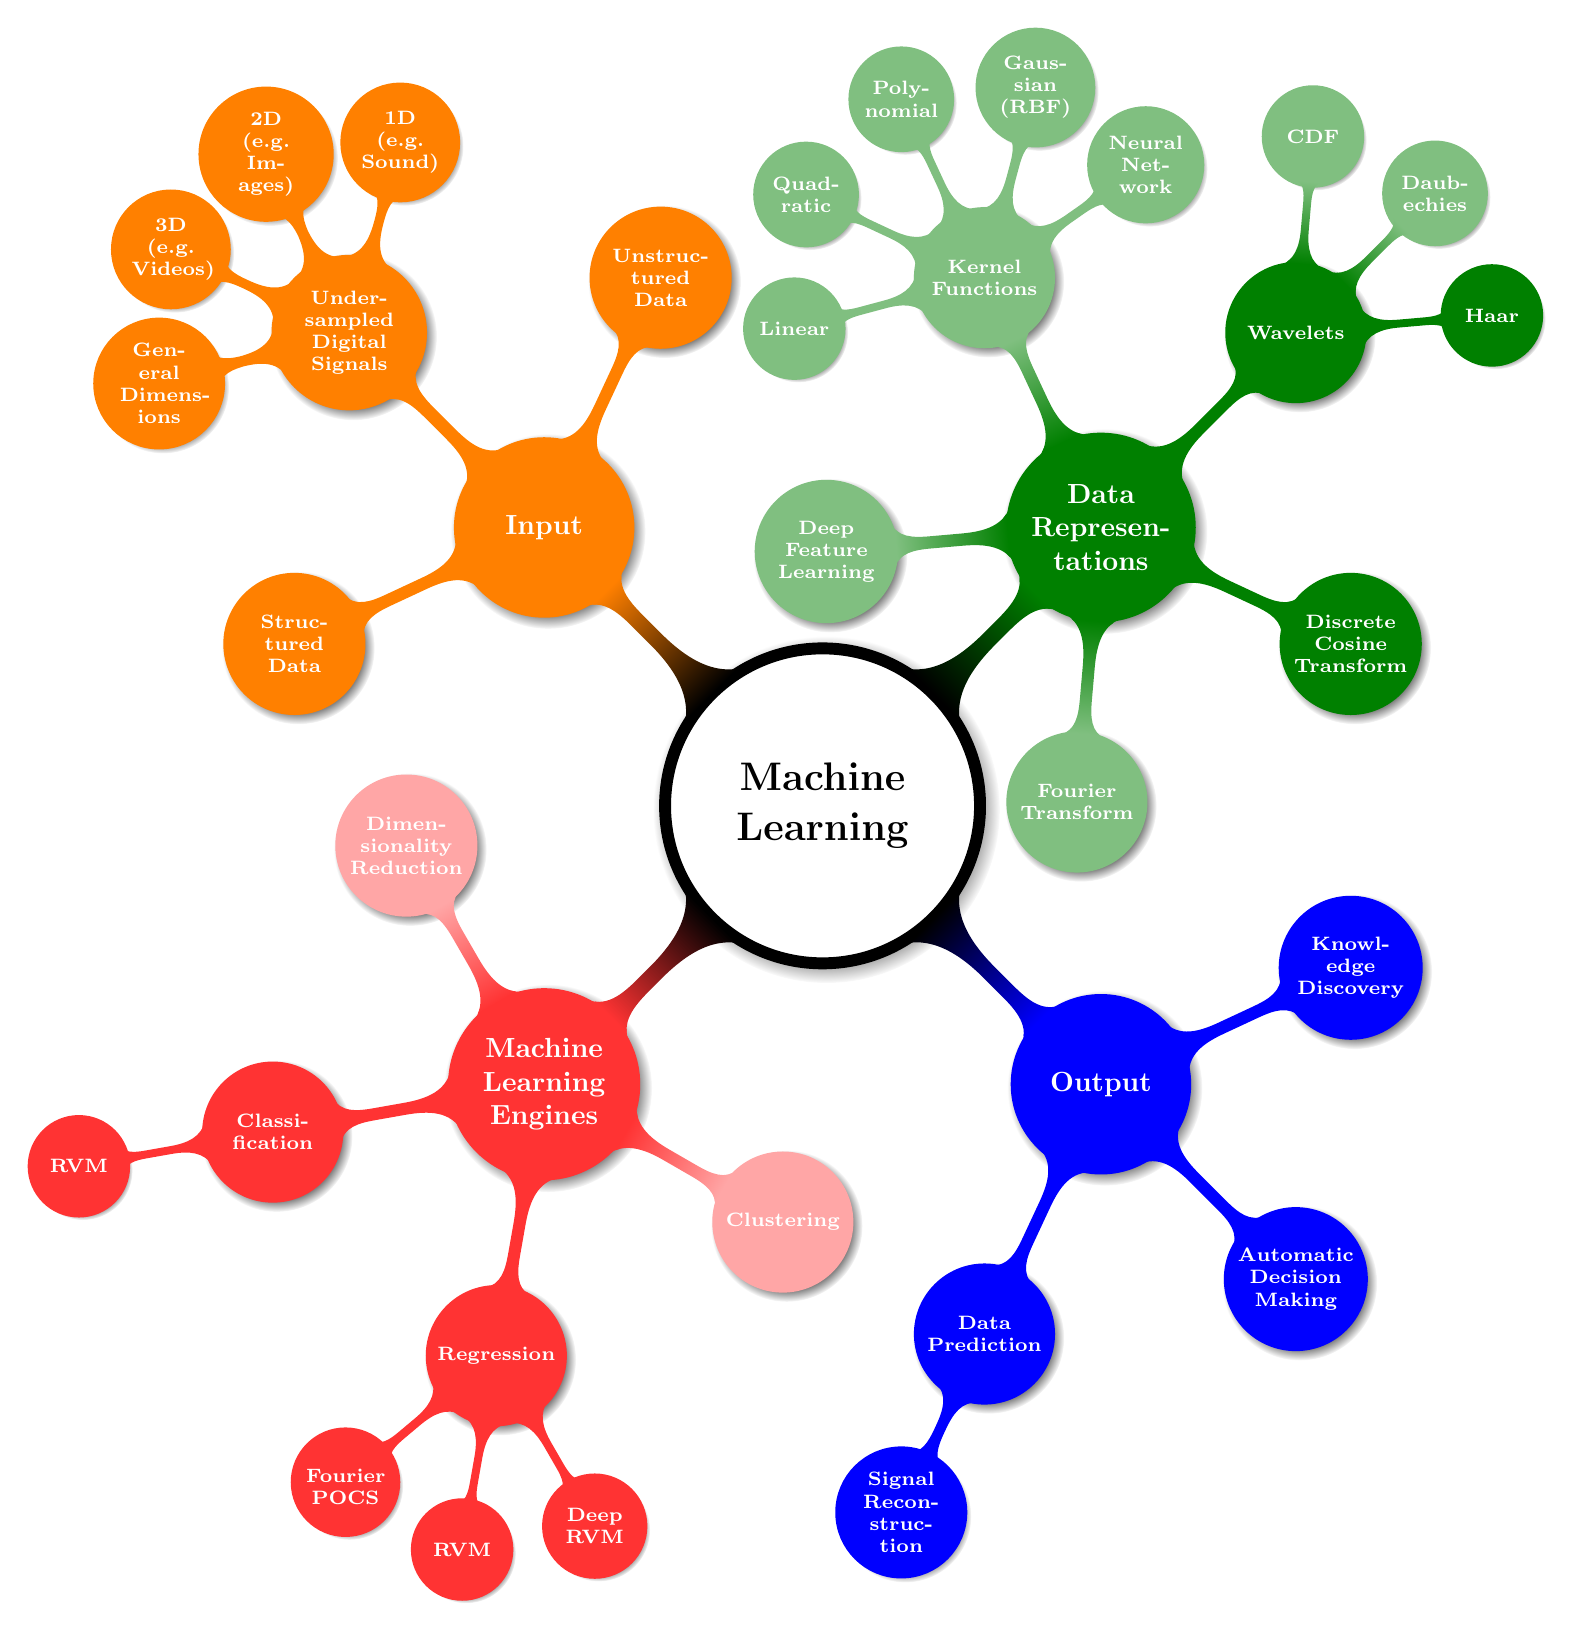
\begin{tikzpicture}[mindmap]
  \begin{scope} [
    every node/.style={concept, circular drop shadow, execute at begin node=\hskip0pt},
    root concept/.append style={
      concept color=black, fill=white, line width=1ex, text=black, font=\Large\bf},
    text=white,
    input/.style={concept color=orange, faded/.style={concept color=orange!50}},
    basis/.style={concept color=green!50!black, faded/.style={concept color=green!50!black!50}},
    engine/.style={concept color=red!80!white, faded/.style={concept color=red!50!white!70}},
    output/.style={concept color=blue, faded/.style={concept color=blue!50}},
    grow cyclic,
    level 1/.append style={level distance=5cm, font=\bf\normalsize, sibling angle = 90},
    level 2/.append style={level distance=3.5cm, font=\bf\scriptsize, sibling angle = 70},
    level 3/.append style={level distance=2.5cm, line width=1ex, font=\bf\scriptsize, sibling angle = 40}]
    \node [root concept]{Machine Learning}    
    %% *** Engine ***
    child [engine] { node {Machine Learning Engines} 
      child [faded] { node{Dimensionality Reduction} }
      child { node {Classification}
        child { node {RVM} }
      }        
      child { node {Regression}
        child { node {Fourier POCS} }
        child { node {RVM} }
        child { node {Deep RVM} }          
      }              
      child [faded] { node{Clustering} }
    }    
    %% *** Output ***
    child [output] { node {Output} 
      child { node{Data Prediction}
        child { node{Signal Reconstruction} }
      }
      child { node{Automatic Decision Making} }
      child { node{Knowledge Discovery} }
    }
    %% *** Basis ***
    child [basis] { node {Data Representations}
      child [faded] { node {Fourier Transform} }
      child { node{Discrete Cosine Transform} }
      child { node{Wavelets} 
        child { node{Haar} }
        child [faded] { node{Daub\-echies} }
        child [faded] { node{CDF} }
      }
      child [faded] { node {Kernel Functions}
        child { node {Neural Network} }
        child { node {Gaussian (RBF)} }
        child { node {Polynomial} }
        child { node {Quad\-ratic} }
        child { node {Linear} }
      }
      child [faded] { node {Deep Feature Learning} }
    }
    %% *** Input ***
    child [input] { node {Input}
      child { node {Unstructured Data} }
      child { node {Undersampled Digital Signals} 
        child { node{1D (e.g. Sound)} }
        child { node{2D (e.g. Images)} }
        child { node{3D (e.g. Videos)} }
        child { node{General Dimens\-ions} }
      }
      child { node {Structured Data} }
  };
\end{scope}
\end{tikzpicture}

\end{document}


%% End of file.